\section{Results across Test Conditions}
\label{sec:taxonomy}

\paragraph{Pre-registered hypotheses.}
We pre-registered 16 predictions in five stages before running the corresponding experiments.
Of these, 10 were confirmed, 4 were refuted, and 2 were partially confirmed.
Appendix~\ref{sec:appendix_preregistered} lists the predictions and outcomes; the corresponding experiment identifiers (P14--P19, P21) accompany the results below.

Table~\ref{tab:main} reports the main results across all five backbones and three shift types.
Each column measures a different response to the test conditions. We examine how model ordering changes between columns.

\begin{table}[H]
\centering
\caption{\textbf{Robustness rankings are shift-specific.}
Five backbones evaluated across sensor dropout, cross-city transfer, and
temporal subgroup shift. Values are mean $\pm$ population std over 3 seeds;
lower is better.}
\label{tab:main}
\vskip 0.05in
\resizebox{\linewidth}{!}{%
\begin{tabular}{lcccc}
\toprule
\textbf{Backbone} & \textbf{In-dist MAE (mph)} & \textbf{$\DeltaSensor$ (30\%, norm.)} & \textbf{X-city (norm.)$^{\dagger}$} & \textbf{$\DeltaTemp$ (norm.)} \\
\midrule
DCRNN (fixed diffusion)       & $6.58 \pm 0.03$ & $+0.020 \pm 0.002$ & $0.180 \pm 0.001$ & $+0.087 \pm 0.004$ \\
GRU   (graph-free)            & $7.49 \pm 0.12$ & $+0.025 \pm 0.012$ & $0.278 \pm 0.009$ & $+0.093 \pm 0.003$ \\
MTGNNLight (sparse cosine-sim)& $6.88 \pm 0.11$ & $+0.051 \pm 0.012$ & $0.244 \pm 0.004$ & $+0.075 \pm 0.007$ \\
STGCN (fixed spectral)        & $7.12 \pm 0.05$ & $+0.078 \pm 0.007$ & $0.249 \pm 0.008$ & $+0.093 \pm 0.003$ \\
GWNet (dense adaptive adj)    & $7.85 \pm 0.11$ & $+0.088 \pm 0.017$ & $0.268 \pm 0.006$ & $+0.094 \pm 0.009$ \\
\bottomrule
\end{tabular}}
{\footnotesize $^{\dagger}$Source-only adjacency; METR-LA-stat normalized MAE on PEMS-BAY.}
\end{table}

\paragraph{Sensor dropout.}
GWNet has the largest sensor-dropout increase in the canonical bank. DCRNN and
GRU have the smallest deltas, while MTGNNLight is markedly less fragile than
GWNet despite also learning topology. Learning a graph is therefore not enough to explain the fragility;
the relevant contrast is sparse learned routing versus dense all-pairs softmax. Capacity controls reduce but do not remove the GWNet
gap (Table~\ref{tab:consolidated}; Appendix~\ref{sec:appendix_stronger_gwnet}).
Dropping high-degree sensors increases GWNet's gap but reduces DCRNN's. This difference is consistent with GWNet relying more heavily on routes through these sensors.
The ranking also depends on corruption type: at 30\% affected channels,
GWNet's healthy-sensor increase is $+0.16$ mph for noise but $+1.96$ mph
for bias, compared with DCRNN's $+0.28$ and $+1.00$ mph, respectively
(Appendix~\ref{sec:appendix_corruption_suite}).

\paragraph{Cross-city transfer under matched structural access.}
Under source-only adjacency, DCRNN is the strongest canonical-bank transfer
baseline. STGCN, also a fixed-graph model, loses much of its advantage when target topology is withheld and then performs similarly to GWNet. The DCRNN advantage also holds on a second
city pair, while padding sensitivity changes absolute MAE but not the ordering
(Table~\ref{tab:consolidated}; Appendix~\ref{sec:appendix_no_pad_sensitivity}).
The GRU baseline is useful here because it removes graph mismatch entirely and
still transfers worst in the canonical bank. Cross-city robustness therefore
does not come from ignoring structure; it depends on how the source-city
structure is used when the target graph is unavailable. A limited fine-tuning comparison is reported in Appendix~\ref{sec:appendix_fewshot}.

\paragraph{Temporal subgroup shift (canonical bank).}
The canonical models have similar weekend/weekday gaps, with much less separation than under sensor dropout or city transfer. None uses explicit time-of-day or day-of-week inputs, and graph type does not explain the small differences. The extended models show larger differences whose interpretation depends on the error metric (\S\ref{sec:extended}).

Appendix Table~\ref{tab:consolidated} summarizes the capacity, source-adjacency, structured-dropout, and horizon comparisons.

\subsection{AGCRN, MegaCRN, and STAEformer}
\label{sec:extended}

Table~\ref{tab:extended} compares AGCRN, MegaCRN, and STAEformer with DCRNN. All use the same METR-LA split and remain frozen during evaluation.

\begin{table}[H]
\centering
\caption{\textbf{Adaptive-relation models under the three test conditions.}
Clean MAE follows each architecture's standard masked-MAE convention; shift
columns use the same normalized protocol as Table~\ref{tab:main}.}
\label{tab:extended}
\vskip 0.05in
\resizebox{\linewidth}{!}{%
\begin{tabular}{lcccc}
\toprule
\textbf{Model} & \textbf{Clean MAE (mph)} & \textbf{$\DeltaSensor$ (30\%, norm.)} & \textbf{Cross-city (src, norm.)} & \textbf{$\DeltaTemp$ (norm.)} \\
\midrule
AGCRN      & $4.09 \pm 0.02^{\dagger}$ & $+0.019 \pm 0.001$ & $0.206 \pm 0.009$ & $+0.061 \pm 0.008$ \\
MegaCRN    & $3.04 \pm 0.06^{\dagger}$ & $-0.048 \pm 0.027$ & $0.163 \pm 0.003$ & $+0.734 \pm 0.019$ \\
STAEformer & $2.93 \pm 0.01^{\dagger}$ & $+0.015 \pm 0.001$ & $0.223 \pm 0.008$ & $+0.750 \pm 0.003$ \\
\midrule
DCRNN (ref) & $6.58 \pm 0.03$ & $+0.020 \pm 0.002$ & $0.180 \pm 0.001$ & $+0.087 \pm 0.004$ \\
\bottomrule
\end{tabular}}
\vskip 0.05in
{\footnotesize $\dagger$ Masked MAE (target $> 0$); DCRNN uses plain MAE.
Cross-family clean-performance ranking is not meaningful due to this convention difference.}
\end{table}

\paragraph{Sensor dropout.}
AGCRN and STAEformer stay near DCRNN on sensor dropout, so GWNet's result
cannot be read as ``adaptive graphs are fragile.'' The distinction is dense
all-pairs softmax (Eq.~\ref{eq:adaptive_adj}) versus node-specific or
attention-mediated relations. MegaCRN's negative delta is non-monotonic in
dropout ratio and is attributed to adjacency-mediated smoothing toward a weekday prior (\S\ref{sec:polish_ablations}), not as direct dropout
robustness.

\paragraph{Cross-city transfer.}
MegaCRN attains the lowest source-stat cross-city MAE, so DCRNN's lead
in zero-shot transfer holds only within the canonical bank. AGCRN and STAEformer fall between DCRNN and GWNet.

\paragraph{Temporal subgroup shift.}
In physical units, MegaCRN and STAEformer have \emph{lower} weekend error:
their weekend-minus-weekday gaps are $-0.594\pm0.051$ and
$-0.612\pm0.002$ masked mph, respectively. AGCRN's gap is
$+0.750\pm0.013$ mph. The normalized gaps in Table~\ref{tab:extended} are
positive for all three models. Thus the large normalized gaps do not establish
greater physical-error fragility: scaling and target masking reverse the sign
for two models (Appendix~\ref{sec:appendix_temporal_absolute}). Covariate
interventions address the normalized gap, not this absolute-error ranking.

\paragraph{Comparison across shifts.}
The adaptive-relation models differ across deployment settings
(Figure~\ref{fig:shift_profiles}): AGCRN and STAEformer match DCRNN under
sensor dropout, MegaCRN leads source-normalized cross-city transfer, and
temporal comparisons depend on the reporting convention. Routing concentration
tracks sensor-dropout sensitivity even when clean accuracy and cross-city
ranking move in different directions. The sensor-dropout ranking is specific
to silent zero-masking; under last-observed-value carry-forward
(LOCF) with the true failure mask, the four backbones in the comparison recover
${\geq}97\%$ of the gap (Appendix~\ref{sec:appendix_imputation}), so the
practical impact of GWNet's fragility depends on the deployment pipeline's
imputation policy. The main conclusions are drawn from METR-LA as the source
city; PEMS04 is used only for targeted source-city replication, not as a full
third-source benchmark (\S\ref{sec:discussion}).

\begin{figure}[H]
\centering
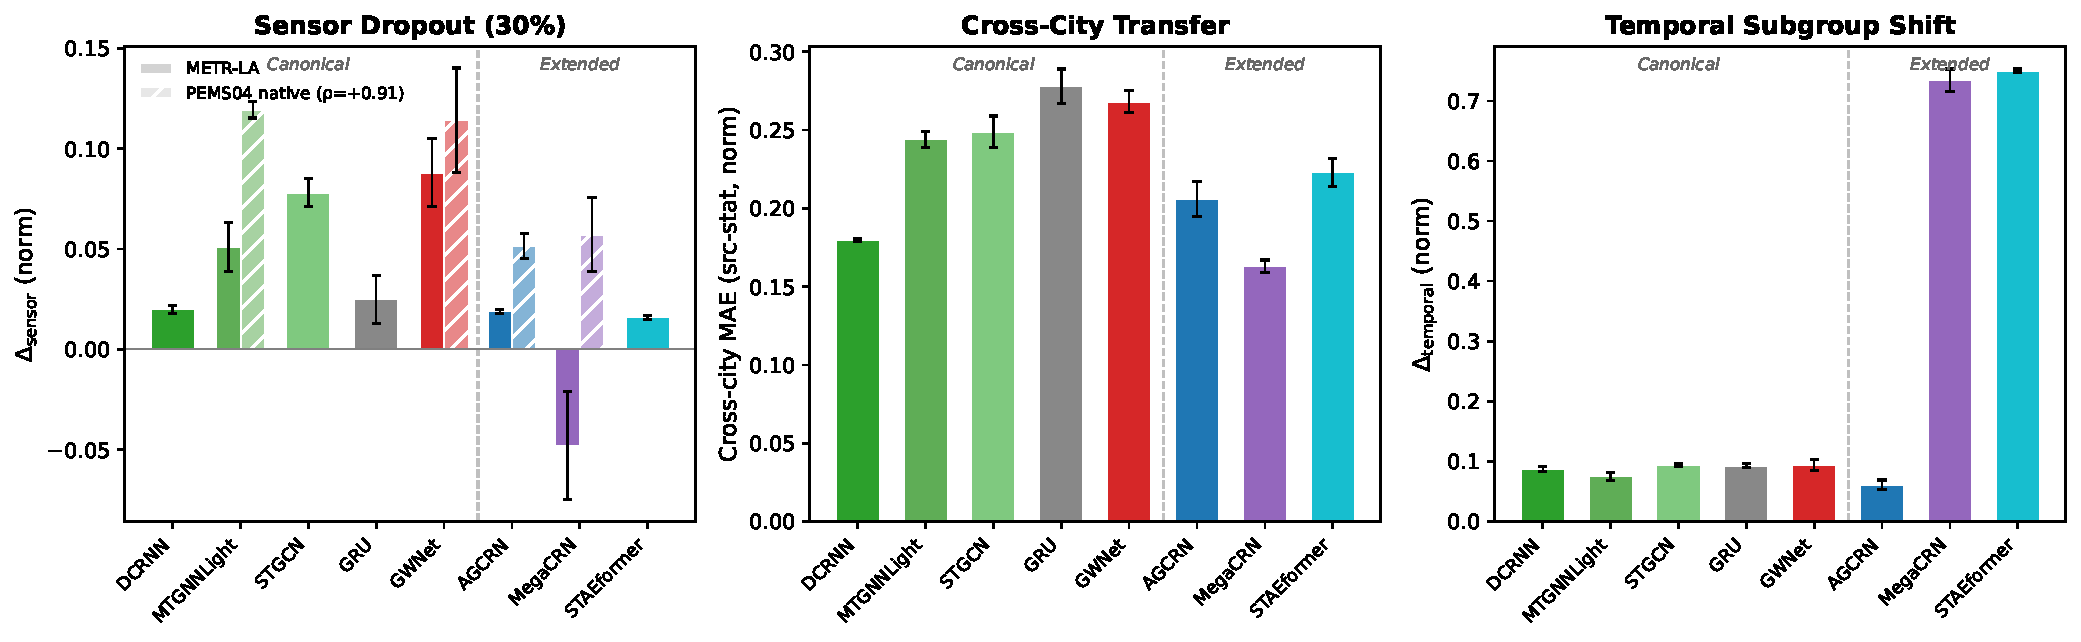
\includegraphics[width=\textwidth]{figures/shift_profiles.pdf}
\caption{\textbf{Sensor-dropout, transfer, and temporal errors.}
Sensor and city panels show all eight backbones; the dashed line separates
the canonical and extended banks. Hatched bars show PEMS04-native replication.
The temporal panel shows masked-mph gaps for the three extended models:
MegaCRN and STAEformer have lower weekend error despite positive normalized
gaps. Error bars are population std over three seed-level means.}
\label{fig:shift_profiles}
\end{figure}
